\section{The Rust Embedded Library}
\label{sec:rel}

As mentioned in \autoref{sec:rsl}, \gls{rsl} is built with the assumption that the application is running on an \gls{os}.
This section presents some of the libraries provided by {\rust} that can be used in a bare-metal system, and how and why they are composed into what we refer to as the \gls{rel}, shown in \autoref{fig:rust:rel}.
\gls{rel} is, unlike \gls{rsl}, not built as a facade, in fact, it is not implemented by us at all.
It is just a way to provide a well-defined definition of the {\rust} library in an embedded system.

\begin{figure}[H]
  \begin{center}
    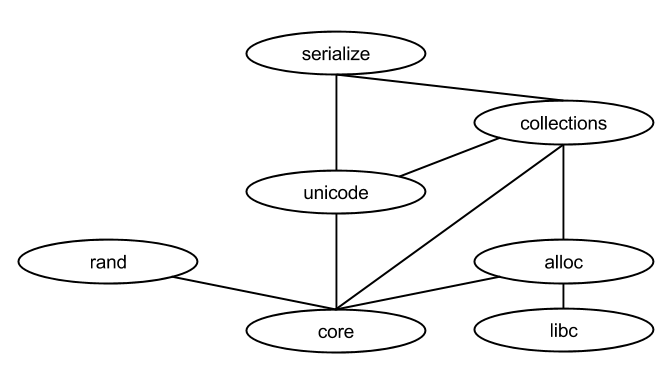
\includegraphics[scale=0.3]{figures/background/rust/embedded-rust-lib.png}
  \end{center}
  \caption{{\rust} Embedded Library}
  \label{fig:rust:rel}
\end{figure}

\subsection{The Core Library}
\label{sec:rust:core}

As described in \autoref{sec:rcl}, the \gls{rcl} defines the \emph{core} functionality of the {\rust} language.
The \gls{rcl} does not have any library dependencies, but in order to use the library without \gls{rsl} a few definitions are needed.
These definitions are given in \autoref{tab:core:definitions}.

\begin{table}[H]
  \centering
  \begin{tabular}{l | l}
    \textbf{Functions} & \textbf{Description} \\
    \hline
    \code{memcpy, memcmp, memset} & Basic memory management \\
    \code{rust\_begin\_unwind}    & Handles panicking \\
    \hline
  \end{tabular}
  \caption{External dependencies of \gls{rcl}}
  \label{tab:core:definitions}
\end{table}

The memory management functions given in \autoref{tab:core:definitions} are provided by \lib{newlib} and are exposed through the \lib{startup} library described in \autoref{sec:startup}.
The \code{rust\_begin\_unwind} is also defined in \lib{startup}, but the implementation is only an infinite loop to aid debugging.
In contrast, the definition of \code{rust\_begin\_unwind} given in \gls{rsl} will abort the program and print an error message.
\concept{Panicking} is {\rust}'s way of unwinding the currently executing thread, ultimately resulting in the thread being terminated.

\subsection{The Allocation Library}
\label{sec:rust:allocation}

Heap allocation is introduced in a library called \lib{alloc}.
The library defines the managed pointer, \code{Box}, which is {\rust}'s main means of allocating memory on the heap.
Also, the allocation library defines the types \code{Rc} and \code{Arc}, which are {\rust}'s \emph{reference counted} and \emph{atomically reference counted} heap pointers.
The allocation library is by default dependent on \lib{libc}, but this dependency can be broken by supplying the \flag{--cfg feature="external\_funcs"} flag to the compilation process.
When breaking this dependency the allocation library requires the functions in \autoref{tab:alloc:external-funcs} to be defined.

\begin{listing}[H]
  \begin{rustcode}
fn rust_allocate(usize, usize) -> *mut u8;
fn rust_deallocate(*mut u8, usize, usize);
fn rust_reallocate(*mut u8, usize, usize, usize) -> *mut u8;
  \end{rustcode}
  \caption{External dependencies of the \lib{alloc} library}
  \label{tab:alloc:external-funcs}
\end{listing}

\subsection{The Collection Library}

The {\rust} \lib{collections} library provides general purpose data structures.
Out of these data structures, the \code{Vector}, a growable heap allocated list, and the \code{String}, heap-allocated mutable strings, are the most notable.
As one would guess, the collection library depends on the allocation library as it needs to allocate memory on the heap.
The \lib{unicode} dependency is due to the \code{String} type is defined as a valid UTF-8 string.
